% An algebraic hexagon: the points x^{(1)},...,x^{(6)} clockwise from the top
% on a regular hexagon of circumradius 2.1, and the lines p^{(ij)} through
% consecutive points, drawn past both points so that they read as lines and
% not as bounded edges. Point labels sit radially inside, line labels outside
% the middle of their line.
% Points in the dark blue and lines in the yellow of the taxa of the trees.
\begingroup
\definecolor{g2TaxonBlue}{HTML}{1676A3}
\definecolor{g2TaxonYellow}{HTML}{E39A24}
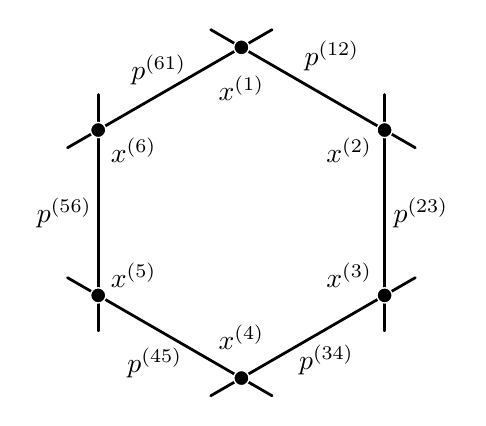
\begin{tikzpicture}[x=1cm,y=1cm,baseline=(current bounding box.center),
  hexagon line/.style={draw=black,line width=1pt,line cap=round},
  hexagon point/.style={circle,fill=black,draw=white,line width=.5pt,inner sep=0pt,minimum size=5.5pt},
]
% The negative shortenings are not in the bounding box: the ends of the lines.
\path (-2.24,-2.35) rectangle (2.24,2.35);
\foreach \i/\a in {1/90,2/30,3/-30,4/-90,5/-150,6/150}
  \coordinate (x\i) at (\a:2.1);
\foreach \i/\j in {1/2,2/3,3/4,4/5,5/6,6/1}
  \draw[hexagon line,shorten <=-.45cm,shorten >=-.45cm] (x\i)--(x\j);
\foreach \i/\a in {1/90,2/30,3/-30,4/-90,5/-150,6/150} {
  \node[hexagon point] at (x\i) {};
  \node at (\a:1.58) {$x^{(\i)}$};
}
\foreach \l/\a/\r in {12/60/2.3,23/0/2.28,34/-60/2.16,45/-120/2.2,56/180/2.25,61/120/2.1}
  \node at (\a:\r) {$p^{(\l)}$};
\end{tikzpicture}
\endgroup
